\documentclass{sigchi}

% Use this command to override the default ACM copyright statement (e.g. for preprints). 
% Consult the conference website for the camera-ready copyright statement.


%% EXAMPLE BEGIN -- HOW TO OVERRIDE THE DEFAULT COPYRIGHT STRIP -- (July 22, 2013 - Paul Baumann)
% \toappear{Permission to make digital or hard copies of all or part of this work for personal or classroom use is 	granted without fee provided that copies are not made or distributed for profit or commercial advantage and that copies bear this notice and the full citation on the first page. Copyrights for components of this work owned by others than ACM must be honored. Abstracting with credit is permitted. To copy otherwise, or republish, to post on servers or to redistribute to lists, requires prior specific permission and/or a fee. Request permissions from permissions@acm.org. \\
% {\emph{CHI'14}}, April 26--May 1, 2014, Toronto, Canada. \\
% Copyright \copyright~2014 ACM ISBN/14/04...\$15.00. \\
% DOI string from ACM form confirmation}
%% EXAMPLE END -- HOW TO OVERRIDE THE DEFAULT COPYRIGHT STRIP -- (July 22, 2013 - Paul Baumann)


% Arabic page numbers for submission. 
% Remove this line to eliminate page numbers for the camera ready copy
 \pagenumbering{arabic}


% Load basic packages
%\usepackage{biblatex}
\usepackage{balance}  % to better equalize the last page
\usepackage{graphics} % for EPS, load graphicx instead
\usepackage{times}    % comment if you want LaTeX's default font
\usepackage{url}      % llt: nicely formatted URLs
\usepackage{listings}
\usepackage[T1]{fontenc}
\usepackage[utf8]{inputenc}
\usepackage{microtype}

\lstset{basicstyle=\footnotesize\ttfamily,breaklines=true}
% llt: Define a global style for URLs, rather that the default one
\makeatletter
\def\url@leostyle{%
  \@ifundefined{selectfont}{\def\UrlFont{\sf}}{\def\UrlFont{\small\bf\ttfamily}}}
\makeatother
\urlstyle{leo}


% To make various LaTeX processors do the right thing with page size.
\def\pprw{8.5in}
\def\pprh{11in}
\special{papersize=\pprw,\pprh}
\setlength{\paperwidth}{\pprw}
\setlength{\paperheight}{\pprh}
\setlength{\pdfpagewidth}{\pprw}
\setlength{\pdfpageheight}{\pprh}

% Make sure hyperref comes last of your loaded packages, 
% to give it a fighting chance of not being over-written, 
% since its job is to redefine many LaTeX commands.
\usepackage[pdftex]{hyperref}
\hypersetup{
pdftitle={SIGCHI Conference Proceedings Format},
pdfauthor={LaTeX},
pdfkeywords={SIGCHI, proceedings, archival format},
bookmarksnumbered,
pdfstartview={FitH},
colorlinks,
citecolor=black,
filecolor=black,
linkcolor=black,
urlcolor=black,
breaklinks=true,
}

% create a shortcut to typeset table headings
\newcommand\tabhead[1]{\small\textbf{#1}}


% End of preamble. Here it comes the document.
\begin{document}

\title{Graphical Structured Temporal Programming for Interactive Applications}

\numberofauthors{3}
\author{
  \alignauthor 1st Author Name\\
    \affaddr{Affiliation}\\
    \affaddr{Address}\\
    \email{e-mail address}\\
    \affaddr{Optional phone number}
  \alignauthor 2nd Author Name\\
    \affaddr{Affiliation}\\
    \affaddr{Address}\\
    \email{e-mail address}\\
    \affaddr{Optional phone number}    
  \alignauthor 3rd Author Name\\
    \affaddr{Affiliation}\\
    \affaddr{Address}\\
    \email{e-mail address}\\
    \affaddr{Optional phone number}
}

\maketitle

\begin{abstract}
  The development of interactive shows and interactive user interfaces for arts \& exhibitions
has traditionally been done with tools that pertain to two broad metaphors. 
Cue-based environments work by making groups of parameters and sending them to remote devices, 
while more interactive applications are generally written in domain-specific 
programming environments, like Max/MSP, Processing or OpenFrameworks.
  In this paper, we argue about the specific issues that arise in such environments, and we present 
i-score : an extensive and collaborative software suite that bridges
the gap between time-based, logic-based and flow-based interactive application authoring tools. 
This is done in a single cohesive graphical user interface, built upon a few simple and novel primitives.
  i-score allows the creation of software meant for operation in a large parameter space, 
and enables artists to express easily both temporal logic and structured programming, 
with facilities for automating and applying transformations to single and multi-dimensional parameters.
\end{abstract}

\keywords{
	Guides; instructions; author's kit; conference publications;
	keywords should be separated by a semi-colon. \newline
	\textcolor{red}{Optional section to be included in your final version, 
  but strongly encouraged.}
}

\category{H.5.m.}{Information Interfaces and Presentation (e.g. HCI)}{Miscellaneous}

See: \url{http://www.acm.org/about/class/1998/}
for more information and the full list of ACM classifiers
and descriptors. \newline
\textcolor{red}{Optional section to be included in your final version, 
but strongly encouraged. On the submission page only the classifiers’ 
letter-number combination will need to be entered.}

\section{Introduction}
This paper presents a paradigm that aims to allow non-programmers 
to conceive interactive applications easily and execute them in production.

The existing software stack is either oriented too much towards the 
cue paradigm, which is useful as long as there is no complex logic involved, 
or towards the programming paradigm, where it is hard to write simple scenarios 
like "move a spotlight in horizontal oscillation for ten seconds; after the first 5 
seconds, if a dancer jumps on the stage, play a sound and increase reverberation steadily as long as the dancer is on stage".

We will first present the current practices on the field, including the depiction of three specific artistic installations revolving around the idea of a computer-controlled orchestration.

We will then explain the paradigm of the i-score software, which allows to express complex scenarios in a single graphical interface. These scenarios involve both temporal logic and structured programming. They can afterwards be deported or even embedded in other tools thanks to a C++ API. 

\subsection{Motivation}
The need for authoring software able to operate in both the temporal and logical domains arises as soon as an artist wants to set-up a show which may have different outcomes according to the actions of the performer, or even of the participants.

\subsection{Use cases}
To explain properly the kind of artistic demeanors we are working with, there will be three case studies.

\paragraph{The Drop}
\paragraph{Klavierstücke XI}
This is a music piece composed in 1957 by Karlheinz Stockhausen.

The interpretation plays a huge part on the piece. It is composed of multiple "segments", a bit longer than musical bars.

The performer starts with one of the segments. When he finishes playing a segment, he chooses another randomly. When he wants to choose a segment that he has already played two times, the music stop.

Hence,  each interpretation is potentially unique.

We can model this programmatically quite easily by maintaining counters for each segment, incrementing the counter when it is played, and having a loop whose looping condition is "no counter is > 2".
% Dire que pour i-score il manque juste la possibilité de créer des données à la volées. Note : pourquoi ne pas simplement ajouter un noeud dans l'arbre lorsqu'il est accédé la première fois (s'il est dans le device local.)

\paragraph{The Runner}
This is an actual museum installation that is located in the Futuroscope, at the city of Poitiers in France. The goal is for children to test their running speed and compare themselves against a leaderboard of the best runners that took the attraction. It is based around two presence detectors, one at the beginning and one at the end of the running lane. However, there is some complexity involved to prevent the children from cheating, for instance by having one of their friends trigger the "finish line" sensor just after they triggered the start sensor. Timeouts are also necessary if a participant starts running but decides to never finish, not triggering the end sensor.

Precisely, the installation can be explained as follows : 
\begin{itemize}
    \item A "welcome" loop that displays a looping video and waits for an interaction.
    \item A main running loop, that starts after the triggering of the start sensor. It begins with a fixed duration announce video that goes "3.. 2.. 1..". While the child runs, there is another video and some music playing. 
    
    If the final sensor is triggered before 5 seconds, it is considered cheating and we break out of the main loop.
    
    If the final sensor is not triggered after 30 seconds, the race is considered abandonnée. 
    
    \item If the main loop does not leave in the "erroring" states, there is a standard finish video that lasts 5 seconds and shows the position of the current run in the podium. After a few seconds, we return to the welcome loop.
    
    \item Overarching all this, there is a topmost loop that regularly checks if the installation is correctly networked with the museum backend. If it's not the case, everything is stopped and a generic "Please call a technician" message is shown.
\end{itemize}

Currently, the whole logic is implemented in Max/MSP. A picture can be seen in fig.~\ref{fig.futuroscope}.

\begin{figure}
    \centering
    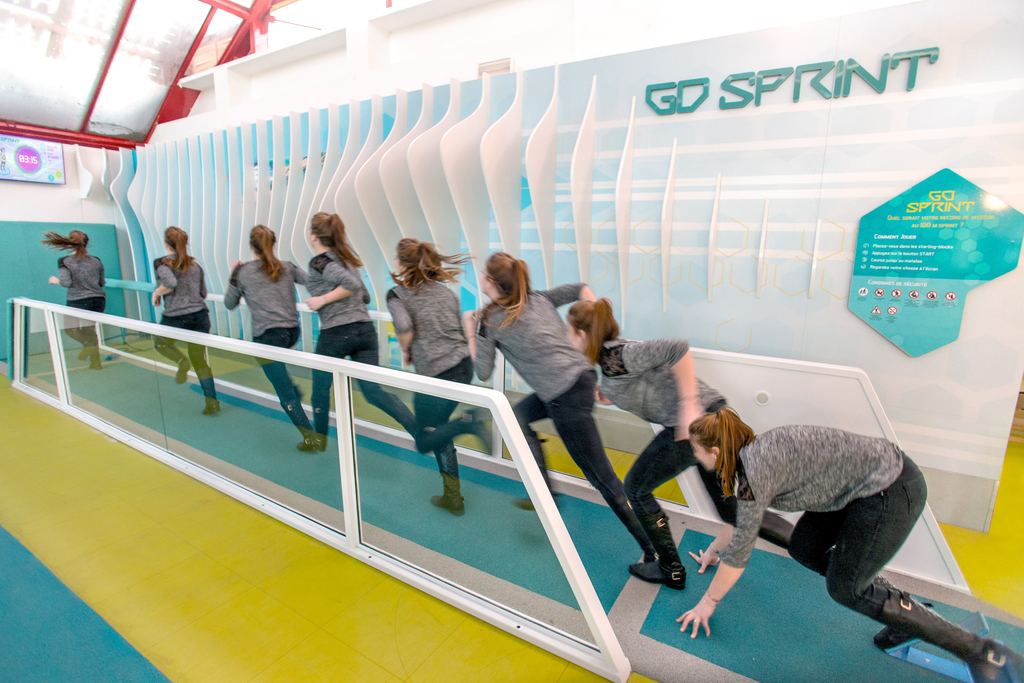
\includegraphics[scale=0.6]{images/futuroscope.jpg}
    \caption{The Runner installation. \tiny{©JL AUDY/FUTUROSCOPE}}
\end{figure}
% Dire que pour i-score il manque juste la possibilité de gérer des "sorties" à tout instant.

\subsection{Existing approaches}
Now that we have exposed the kind of problems that we are tackling, we are going to review the existing methods that have been and are still used to conceive and run interactive applications.

There are mostly three parts : first, the cue-based tools. This is a broad range which can go from extremely specialized software that would for instance only handle video, to more generic solutions that aim to control different kinds of media.

Then, the text-based programming tools. These are programming languages that are dedicated to the task of building interesting interactive applications and their user interfaces.

Then, there are specific flow-control models. i-score fits into this category.

In addition, we will have an overview of document object model paradigms. This is to present the kind of software that i-score is expected to control. % Peut-être mettre ça ailleurs, plus loin ?

\subsubsection{Cue-based environments}
This is the first kind of environment for content creation, and certainly one of the most used for shows, because it mimics the behaviour of real hardware such as lighting consoles.

A cue is a set of data that maps to a certain state on stage. For instance, there would be a cue for the beginning of a new scene in a pièce de théâtre, that would set the lights in the correct positions and colors, and start playing a background music.

In this kind of environment, there is no manifest temporal relationships to speak of: the cue are organized in stacks that will generally follow the expected development of the show. A human is generally present to trigger the correct cues at the correct time, and adjusts if something goes wrong on stage.

An example of cue-based system for show control is given by Kim Youngjae in~\cite{kim_unified_2013}. 

This is also similar to the session view of Ableton Live, with stacks of audio clips that are to be triggered by the performer. Modulo Pi is another hardware and software facility that works with video cues.

These environments, overall, allow to set-up a show very easily - sometimes dragging and dropping the desired cues will be enough. But as soon as there is interactivity involved, this paradigm becomes useless : there is absolutely no flexibility apart from the one provided by a human operator, which may become overwhelmed if too much things happen on stage at the same time.

\subsubsection{Programming-based environments}
At the other range of capabilities lies the full-blown programming languages. They allow complete flexibility over what's happenning. However, very few artists are eager to learn how to program in order to write interactive show; besides, when the show relies heavily on temporal elements, the textual structuration doesn't make the flow of the program easy to understand, as can be seen in fig.~\ref{fig.hardtofollow}.

\begin{figure}
\label{fig.hardtofollow}
\begin{lstlisting}[language=c++]
GlobalState state;

void light1()
{
  state.at("/light/r").set(255);
  usleep(200000);    
  state.at("/light/r").set(0);
  for(int i = 0; i < 100; i++)
  {
    if(state.at("/sound/volume") > 50)
      state.at("/light/g").set(i);        
    state.at("/light/b").set(255 - i);
    usleep(32000);
  }
}

void scenario()
{
  state.at("/sound").set(true);
  light1();
  usleep(10000);
  light1();
}
\end{lstlisting}
\caption{A trivial light-changing program. However, the lack of cohesion between the code's organization and the temporal behaviour makes the development of the scenario hard to visualize. Time, logic and data are highly coupled, which makes it even harder to follow.}
\end{figure}

The programmer also needs to keep track of the available data and devices that he can access; this is commonly achieved by using god objects that represent the external devices's state or something akin to haskell's World State concept. Else, a state-keeping object has to be passed across most of the method and function calls, which incurs a certain cost on the complexity of such software. Another common problematic is the method used to represent external devices. Some libraries will rather try to implement everything with the language's primitives and structures. Hence, an address of a device would be represented by a tree-like structure. Other would take an approach closer to a domain-specific language, by specifying the addresses in textual format that are to be parsed behind the scene. 

Besides, another problem is reusability : most of the interactive applications are to be used once and then discarded since they are most of the time very different. Libraries exist, but even then they are generally customized by the final application author. Hence, any system wishing to improve on the current state of affairs would have to provide easy-to-use library facilities.

Finally, the standard primitive for parallelization, threads, is highly unpractical to use because of the indeterminism of the operating system's scheduler. Other programming paradigms, like reactive programming, offers better tools to solve this problem.

For instance, one can write such software with ActionScript (part of the Adobe Flash environment), Processing (a set of multimedia libraries based on Java) and OpenFrameworks, which is to C++ what Processing is to Java\cite{noble2009programming}. These languages or frameworks are general-purpose, but contain a lot of multimedia-oriented tools, to playback and modify video, or create particle systems. 

Some domains have more specific tools : for instance, the LISP community has produced a wealth of languages able to represent interactive music (source).


\subsubsection{Flow control models}

* First present the raw time models, as well as the formal models for i-score

* Then present more advanced software / toolkits


 % du tout temporel au tout logique en passant par systèmes réactifs ?
Max, PureData, React.[...], Integra Live (qui est plutôt orienté son), Unity \& envs de jeu, etc. (revoir slides), Chronic (cf. téléchargements), OpenMusic, Antescofo (et Ascograph), logiciels de la conférence sur appli réactives (cf. slack).

OpenMusic : pas d'exécution.

MEF++\cite{ackermann_direct_1994} : framework pour applications interactives.

Temps souple\cite{song_interactive_1999}


\subsubsection{Document models and application description} % bof ici
CORBA, DBus, DOM HTML, DOM Qt, DOM Jamoma...


\section{A model for orchestration}
We will present our constructs by starting with the purely temporal ones, 
and then extend to the constructs relevant in a structured programming context.
Finally we will see how data is handled.

This model has evolved through many stages of refinement, first starting as an application of 
Allen's relationships and moving on to NTCCs, Petri nets, finite automatons, and reactive languages.

\subsection{Specification of temporal relationships}\label{sec.temporal}
The first required primitive is the one able to depict a duration.

We shall call it a time constraint.

The time constraint is not necessarily a fixed duration : to allow for interactiveness, 
we must allow it to represent a range, or span of time. For instance, a time constraint may last between 3 and 5 seconds.

Then, we introduce a mean to synchronize multiple time constraints : a time node. 

This allows multiple time constraints to exist both serially, and in parallel. 

avec tout ça je devrais pourvoir m’en sortir ! merci.
du coup je m’y colle en début de semaine prochaine et on pourrait se réunir le jeudi 22 ou vendredi 23 à paris ?


\subsection{Structured temporal programming}
Maintenant que nous avons des primitives permettant de décrire l'écoulement du temps, nous introduisons les éléments s'apparentant à la programmation structurée.

La base est la conditionnelle. Dans notre cas, nous aimerions dire : cette contrainte temporelle ne s'exécute que si tel paramètre a atteint cette valeur.

Du fait de la présence de logique temporelle, il y a deux cas de conditions : 
- Les conditions qui ne prennent pas le temps en compte. Elles sont vraies ou fausses, et la chose qui compte est leur valeur au moment ou elles seront évaluées. Elles n'ont d'influence que sur le futur.
- Les conditions qui contrôlent le flot du temps. Elles ont le pouvoir de déclencher des intervalles lorsqu'elles passent à vrai. C'est pour cela que nous avons besoin d'avoir un minimum et un maximum à nos contraintes temporelles. Elles ont donc aussi une influence sur des contraintes temporelles précédentes : on dirait par exemple : "cette contrainte dure *jusqu'à ce que la condition soit vraie". On peut ainsi faire durer une contrainte à l'infini en mettant une condition "faux". Ceci permet d'écrire des applications avec un fonctionnement "moteur", qui ne sont pas sensées s'arrêter.

Nous séparons ces deux cas en deux éléments de syntaxe de notre langage : l'évènement pour le premier, et le trigger pour le second.

Les deux font interface entre les contraintes et les noeuds temporels.

À partir de là, nous pouvons considérer la notion de boucle. Pour cela, il est nécessaire de bien clarifier la séparation entre les données spécifiées par l'auteur, et le résultat de l'exécution.

Quand un auteur ou programmeur spécifie une boucle, il décrit un motif général qui est voué à être répété. Cependant, à chaque itération des cas différents peuvent arriver : 

\begin{lstlisting}
while t < 100
  if a
    [...] short iteration [...]
  else
    [...] long iteration [...]           
\end{lstlisting}

Dans notre cas, nous avons donc besoin d'une contrainte souple pour pouvoir avoir des boucles intéressantes. 

On décrit donc la boucle comme une paire (noeud temporel, contrainte). La contrainte est des deux côtés du noeud temporel : une fois qu'elle a été lue, elle peut être re-lue depuis le début, sachant que l'on progresse dans l'écoulement du temps.


\section{From structure to content}
Maintenant que nous avons établi l'intégralité des éléments nécessaires à une structuration logique et temporelle, nous nous intéressons aux données.

Comme cela a pu être vu en section~\ref{sec.temporal}, nous possédons deux primitives temporelles : une pour les durées et une pour les instants.

Il y a deux points de vue possibles : le premier est que le temps doit être traité comme un continuum : un instant n'a pas d'existence propre et on ne peut que l'approcher comme on approcherait un élément dans un ensemble dense. Ceci permet de raisonner simplement sur des problématiques de positionnement d'éléments par rapport au temps.

Néanmoins, il est parfois utile de briser l'abstraction et d'obtenir le contrôle bas niveau : dans des logiciels audio, c'est par exemple le cas de l'accès à la sample.

Le type de données avec lequel i-score est le plus utilisé est le message OSC. Là aussi, il est nécessaire d'avoir un accès précis au comportement qui s'applique lorsque par exemple, deux courbes se suivent et portent sur la même adresse sans que la fin de la première courbe ait la même valeur que le début de la suivante. Veut-on privilégier une valeur ? Utiliser les deux ? L'utilisateur doit avoir le choix de la valeur envoyée lorsqu'il y a une discrepancy manifeste entre un instant logique dans le scénario, et un instant physique, ordonné par l'horloge d'une carte son ou du cpu.

Dans le logiciel, le type de données que nous manipulons le plus est donc le message, qui associe une valeur à une addresse. Plusieurs messages regroupés forment un état, par analogie avec les cues.

\subsection{Processes}
Pour encapsuler ces données, dans le cadre d'une durée nous choisissons principalement la métaphore du processus. Une contrainte peut contenir un nombre arbitraire de processus; l'interface d'un processus est très simple et permet de décrire des cas complexes. Elle est analogue à un système de passage de messages.

\begin{lstlisting}
    interface Process {
       State state(Time)
    }
\end{lstlisting}

Cela permet à la contrainte de fonctionner de la même manière qu'une tête de lecture : une horloge va envoyer des ticks; à chaque tick le processus doit renvoyer son état. Ce fonctionnement semble fonctionnel pur mais rien n'empêche d'avoir des effets de bord / sauvegarder un état.
Sur un plan théorique (et au niveau de l'exécution) un processus peut être vu comme une succession d'états, néanmoins ce serait une abstraction difficile à manier pour l'auteur, notamment en ce qui concerne les automations.

Il convient donc de noter que les processus peuvent s'arrêter avant leur fin apparente, si par exemple il y a un trigger sur la fin de la contrainte.

Problème des contraintes à l'édition / à l'exécution : certains arguent que tout devrait être souple à l'exécution et rien à l'édition; d'autre le contraire. D'ou plusieurs modes d'édition grâce à un CSP.

\subsection{States}
Les processus ont un sens sur une durée. Cependant, il existe aussi le cas ou nous voudrions envoyer des données à un instant précis : par exemple, pour lancer la lecture d'un média distant.
Pour ce faire, i-score matérialise la notion d'état instantané dans un élément graphique.

Les états sont situés au début et à la fin de chaque contrainte temporelle. Cela permet de spécifier très simplement des interpolations entre deux paramètres, en prenant une capture d'un premier état puis d'un second.

Nous avons donc l'ensemble des éléments de base qui composent ce que l'on nomme un scénario : en reliant contraintes, évènements, états, triggers et noeuds temporels nous pouvons déjà définir ces scénarios complexes, mais linéaires.

Comme nous l'avions dit plus tôt, il est parfois nécessaire de choisir entre deux vues des états : des instants avec une notion d'unicité temporelle, ou bien un point dans un tableau défini par la granularité du scheduler.

Pour ce faire, l'état va enregistrer plusieurs valeurs : 
\begin{itemize}
\item Les valeurs qu'a entré l'utilisateur manuellement à cet instant
\item Les valeurs des processus précédents
\item Les valeurs des processus suivants
\end{itemize}

Ces valeurs peuvent ensuite être prioritisées, et l'utilisateur peut choisir quelles valeurs doivent être synchronisées entre elles en permanence, à la manière d'un système réactif. De même, il est possible de filtrer volontairement sur la répétition d'un même message : on pourrait envoyer ou non le message \verb|/clignote| à un même instant, tout en empêchant de changer plusieurs fois une position à la même valeur. 


Les valeurs des processus peuvent être modifiées de l'extérieur par un système de requête - réponse, si cela est supporté par le plug-in de processus.


% Note : cas ou on a une synchronisation mais la contrainte parente se termine avant

\section{Hiérarchie}
À l'aide de la notion de processus, nous pouvons introduire le concept de hiérarchie. La notion de scénario que nous avons présenté peut être placée dans un processus, qui aura comme spécificité d'avoir un noeud temporel de début. Ainsi, son état peut être récupéré récursivement à chaque instant en fonction des appels du parent.

Par défaut, un document est constitué de deux noeuds temporels, et d'une contrainte intermédiaire qui contient un processus Scénario.
Il aurait été possible d'avoir le cas inverse : l'élément de base aurait pu être un processus scénario dans lequel on commencerait à travailler; cependant avoir une contrainte comme élément parent permet de contrôler la vitesse de lecture globale de manière interne au formalisme. De même, on peut faire "lecture" sur le document en envoyant des messages OSC au noeud temporel de début.

De même, la boucle est implémentée en terme de processus.

La notion de processus est utile car elle permet très simplement de faire des copier-coller, des mute, etc.

\section{Arbres d'états}
Les états se réfèrent la plupart du temps à des périphériques distants : d'autres logiciels compatibles OSC comme Max/MSP ou PureData, ou bien des appareils MIDI.

L'accès se fait via une interface commune, organisée sous forme d'arbre.


% Spécifier possibilités de l'interface Device / Node


L'avantage d'une organisation en arbre est que cela permet de représenter simplement les DOM courants; la majorité des paramètres ont un rôle purement de données, comme par exemple contrôler le volume d'un son. Mais d'autres peuvent avoir des rôles plus complexes et se comporter comme des fonctions qui pourraient elle-même modifier la structure de l'arbre.

% Mettre capture d'écran d'un objet Qt ?

Cette interface peut être simplement réimplémentée. Cependant il faut tenir compte du fait que tous les protocoles n'offrent pas les mêmes capacités : par exemple un arbre MIDI est entièrement fixe car les messages sont fixés dans la spécification MIDI. En revanche un arbre qui correspondrait à un logiciel écrit en Max/MSP serait beaucoup plus dynamique.

Les paramètres présents dans cet arbre peuvent ensuite être accédés depuis tout le logiciel.

Pour l'instant, ils sont donc organisés sous forme d'état global, à l'image d'une base de données. Cependant nous aimerions évoluer vers un état avec une portée locale, peut-être avec un raffinement au niveau des processus (Processus "LocalScope"). Cela rejoindrait le concept d'unité de données de la programmation structurée.

\subsection{Arbre local}
De plus, le document présente lui aussi son propre arbre de paramètres, addressable depuis l'intérieur comme l'extérieur.

Cela permet notamment de se référer au temps qui s'est écoulé à l'exécution pour s'en reservir dans d'autres contraintes. Ces messages sont addressables depuis le réseau; un loopback est implémenté pour un accès local rapide.

Cela permet par exemple de faire des boucles à durée convergente, des canons, et des systèmes en forme de fractale. % donner exemple

\section{Types de données}
En plus des types classiques (entiers, flottants, chaines de caractères, tableaux),  nous offrons deux types de donnée spécifiques et relatifs à l'utilisation temporelle qui est faite.

Le premier est =. = est une aide à l'édition : elle n'a de sens que dans l'état à la fin d'une contrainte et signifie : "s'il existe un message à cette addresse au début de la contrainte, alors prends sa valeur".

Le second est ?. ? prend son sens lors de l'exécution, en permettant d'agir en fonction d'une valeur non connue à l'édition du scénario.

Cela permet par exemple de former un état à partir d'évènements qui dépendent de ce qu'il se produit sur scène, pour faire des mappings; par exemple on pourrait mapper le volume audio à la position d'un danseur sur scène à un instant donné.

\section{Transformations et chaînage}
Perspective : transformations appliquées à une boîte

\section{Processus modèles de données}
Maintenant que nous avons présenté les éléments principaux du modèle temporel, il est temps de se concentrer sur des extensions spécialisées adaptées à des cas particuliers de gestion des données.

\subsection{Automations}
L'élément le plus important de tout séquenceur ou logiciel d'animation est l'automation.

L'automation permet d'avoir un comportement évolutif dans le temps, la plupart du temps continu.

L'automation est une fonction qui à un instant associe un état.

Nous avons essayé de pousser le concept de l'automation au maximum dans i-score.

- Mode par points
- Discontinuités
- Interface de segments
- Modes d'édition inspirés de l'existant

La valeur d'un point dans une automation peut être définie par ? (ou = ?).

Futur : automation de chaînes de caractères ?

\subsection{Mappings simples}
Les mappings sont une généralisation de l'automation.

Plutôt que d'associer du temps à un état, nous associons un état à un autre état par une fonction de transfert. Cette fonction est aussi une courbe.

Par exemple, on peut associer la position d'un danseur à la couleur rouge d'un projecteur, puis avec une autre contrainte temporelle, l'associer à la couleur bleue.

% Futur : associer [x; y] à [hue; saturation] 

\subsection{Mappings spatiaux}

Les mappings que nous présentons là sont une première partie des possibilités que l'on peut avoir.

Nous aimerions maintenant étendre nos travaux à des zones définies entièrement dans l'espace. Pour ce faire, nous utilisons la puissance complète des mathématiques à l'aide d'une bibliothèque de CAS. Ainsi, nous pouvons définir des zones à partir de notre arbre de paramètres et travailler sur des données spatiales : que se passe-t-il quand deux zones entrent en collision ?
    
\subsection{Extensibilité}

- Conclusion : analogue à un petit OS spécialisé pour applications multimédia.

\section{Collaboration et répartition}

\section{Shortcomings (et pistes)}
Lors du développement d'i-score, nous avons trouvé diverses pistes qui, nous le pensons, peuvent contribuer à 
faire évoluer le logiciel mais sont encore des problèmes non-résolus.

\subsection{Debugging}
Les scénarios fournis dans i-score sont des programmes; une pratique (hélas) nécessaire en programmation est le déboguage. 

Le déboguage permet généralement de comprendre pourquoi un programme n'a pas fonctionné correctement. Heureusement, ici, nous n'avons pas de problèmes de gestion de mémoire, ou de pointeurs comme dans des langages  bas-niveau comme le C. Néanmoins, dès que la logique du spectacle devient complexe, il est utile de pouvoir comprendre qu'est-ce qui se passe mal.

\paragraph{Time Scrub}
Le premier outil est le time scrub : il permet de se déplacer dans le temps et d'exécuter un élément sans repartir du début. Un problème évident se pose dès que de l'indéterminisme est introduit dans le scénario : comment gérer deux conditions exclusives par exemple ? Des outils simples et linéaires n'ont pas ce problème et peuvent scrubber à tout instant.

Plusieurs possibilités s'ouvrent alors :
\begin{itemize}
    \item Définir des "chemins" par défaut qui doivent être empruntés lors de l'évaluation.
    \item Choisir avant chaque exécution comment chaque condition doit s'exécuter.
    \item Tout ignorer et ne lire qu'en considérant une contrainte.
\end{itemize}

De plus, un problème de déboguage lié aux contraintes temporelles se pose : jusqu'à présent, nous les avons présentées comme un moyen de définir une contrainte lors de l'exécution d'un scénario. Par exemple, dans le cas d'une machine à fumée, nous pouvons spécifier 10 secondes de préchauffage avant de commencer à envoyer la fumée. Dans certains cas, ne pas respecter le temps de préchauffage peut endommager le matériel, il est donc très important de le réaliser à chaque fois.

Cependant, si l'on autorise le déboguage à démarrer à partir de n'importe quel instant, il est possible de détruire le matériel par inadvertance, ce qui n'est pas désiré. Il est donc nécessaire de trouver un moyen de spécifier des contraintes "absolues" ou "nécessaires", possiblement en lisant un paramère qui indique l'état de préchauffe actuelle et lance une contrainte de préchauffage si l'état n'est pas apte à lancer la suite. Cela se rapproche des outils de scripting qui existent par exemple dans gdb.

\paragraph{Visualisation de l'exécution}
Mode simple : on affiche le déroulement du temps.

Mode avancé : les contraintes vont se déplacer dans le temps depuis le début de leur intervalle souple jusqu'à leur fin.

\paragraph{Traces d'exécution}
Enfin, il peut être utile d'obtenir des traces d'exécution après performance. Cela a un intérêt supplémentaire par rapport à une trace d'exécution d'un logiciel standard : par exemple, si la performance était mauvaise et incluait des danseurs, ils peuvent rejouer l'exécution telle qu'elle s'est passée pour comprendre qu'est-ce qui a posé problème. De même, une très bonne performance pourra être réutilisée par la suite si par exemple le spectacle doit être reproduit dans de moins bonnes conditions (par exemple si un des acteurs ne peut être présent).

Il devrait être possible de synchroniser dans une certaine mesure les traces d'exécution avec le document original : ainsi, si une durée est changée dans le document principal, cela peut être répercuté dans les traces, pour garder les conditions qui se sont / ne se sont pas exécutées.

%\paragraph{Simulation d'environnements}
%- Visualisation / simulation du résultat ? 

\subsection{Extensions}
- Scripting plug-in

\section{Evaluation}
- Time to develop artistic installations greatly reduced.

\section{Conclusion}
%% Logiciel ouvert et utilisable (API C++)
%% Perspectives : autres implémentations (FPGA, kdbus, modèle de calcul ?)

\bibliographystyle{SIGCHI-Reference-Format}
\bibliography{base}

\end{document}
